\documentclass[12pt]{article}

\usepackage{fullpage}
\usepackage{fancybox}
\usepackage{graphicx}

\newcommand{\SubSum}{\textsf{\sc SubsetSum}}
\newcommand{\Partition}{\textsf{\sc Partition}}
\newcommand{\SAT}{\textsf{\sc Sat}}
\newcommand{\KITE}{\textsf{\sc Kite}}
\newcommand{\CLIQUE}{\textsf{\sc Clique}}
\newcommand{\CLIS}{\textsf{\sc CliqueIndepSet}}

\newcounter{ques}
\newenvironment{question}{\stepcounter{ques}{\noindent\bf Question \arabic{ques}:}}{\vspace{5mm}}
\newenvironment{solution}{{\noindent\bf Solution:}}{\vspace{5mm}}

\begin{document} 

\begin{center} \Large\bf
COMP 3804 --- Assignment 4 
\end{center} 

\noindent {\bf Due:} Thursday April 6, 23:59.

\vspace{0.5em}

\noindent {\bf Assignment Policy:}
\begin{itemize}
\item Your assignment must be submitted as one single PDF file through
      Brightspace.

\begin{center}
\hfill\shadowbox{
  \begin{minipage}{.90\linewidth}
    {\textsf{Use the following format to name your file:
        \[ {\tt LastName\_StudentId\_a4.pdf}
        \]
      }}
  \end{minipage}
}
\end{center}
\item {\bf Late assignments will not be accepted. I will not reply to
      emails of the type ``my internet connection broke down at
      23:57'' or ``my scanner stopped working at 23:58'', or
      ``my dog ate my laptop charger''.}
\item You are encouraged to collaborate on assignments, but at the level
      of discussion only. When writing your solutions, you must do so
      in your own words.
\item Past experience has shown conclusively that those who do not put
      adequate effort into the assignments do not learn the material and
      have a probability near 1 of doing poorly on the exams.
\item When writing your solutions, you must follow the guidelines below.
      \begin{itemize}
      \item You must justify your answers.
      \item The answers should be concise, clear and neat.
      \item When presenting proofs, every step should be justified.
      \end{itemize}
\end{itemize}

\newpage 

\begin{question}
Write your name and student number.
\end{question}

\begin{solution}

      Ryan Lo (101117765)
\end{solution}

\begin{question}
Let $K \geq 3$ be an integer. A $K$-\emph{kite} is a graph consisting of 
a clique of size $K$ and a path with $K$ vertices that is connected to 
one vertex of the clique; thus, the number of vertices is equal to $2K$. 
In the figure below, the graph with the black edges forms a $5$-kite. 

\begin{center}
     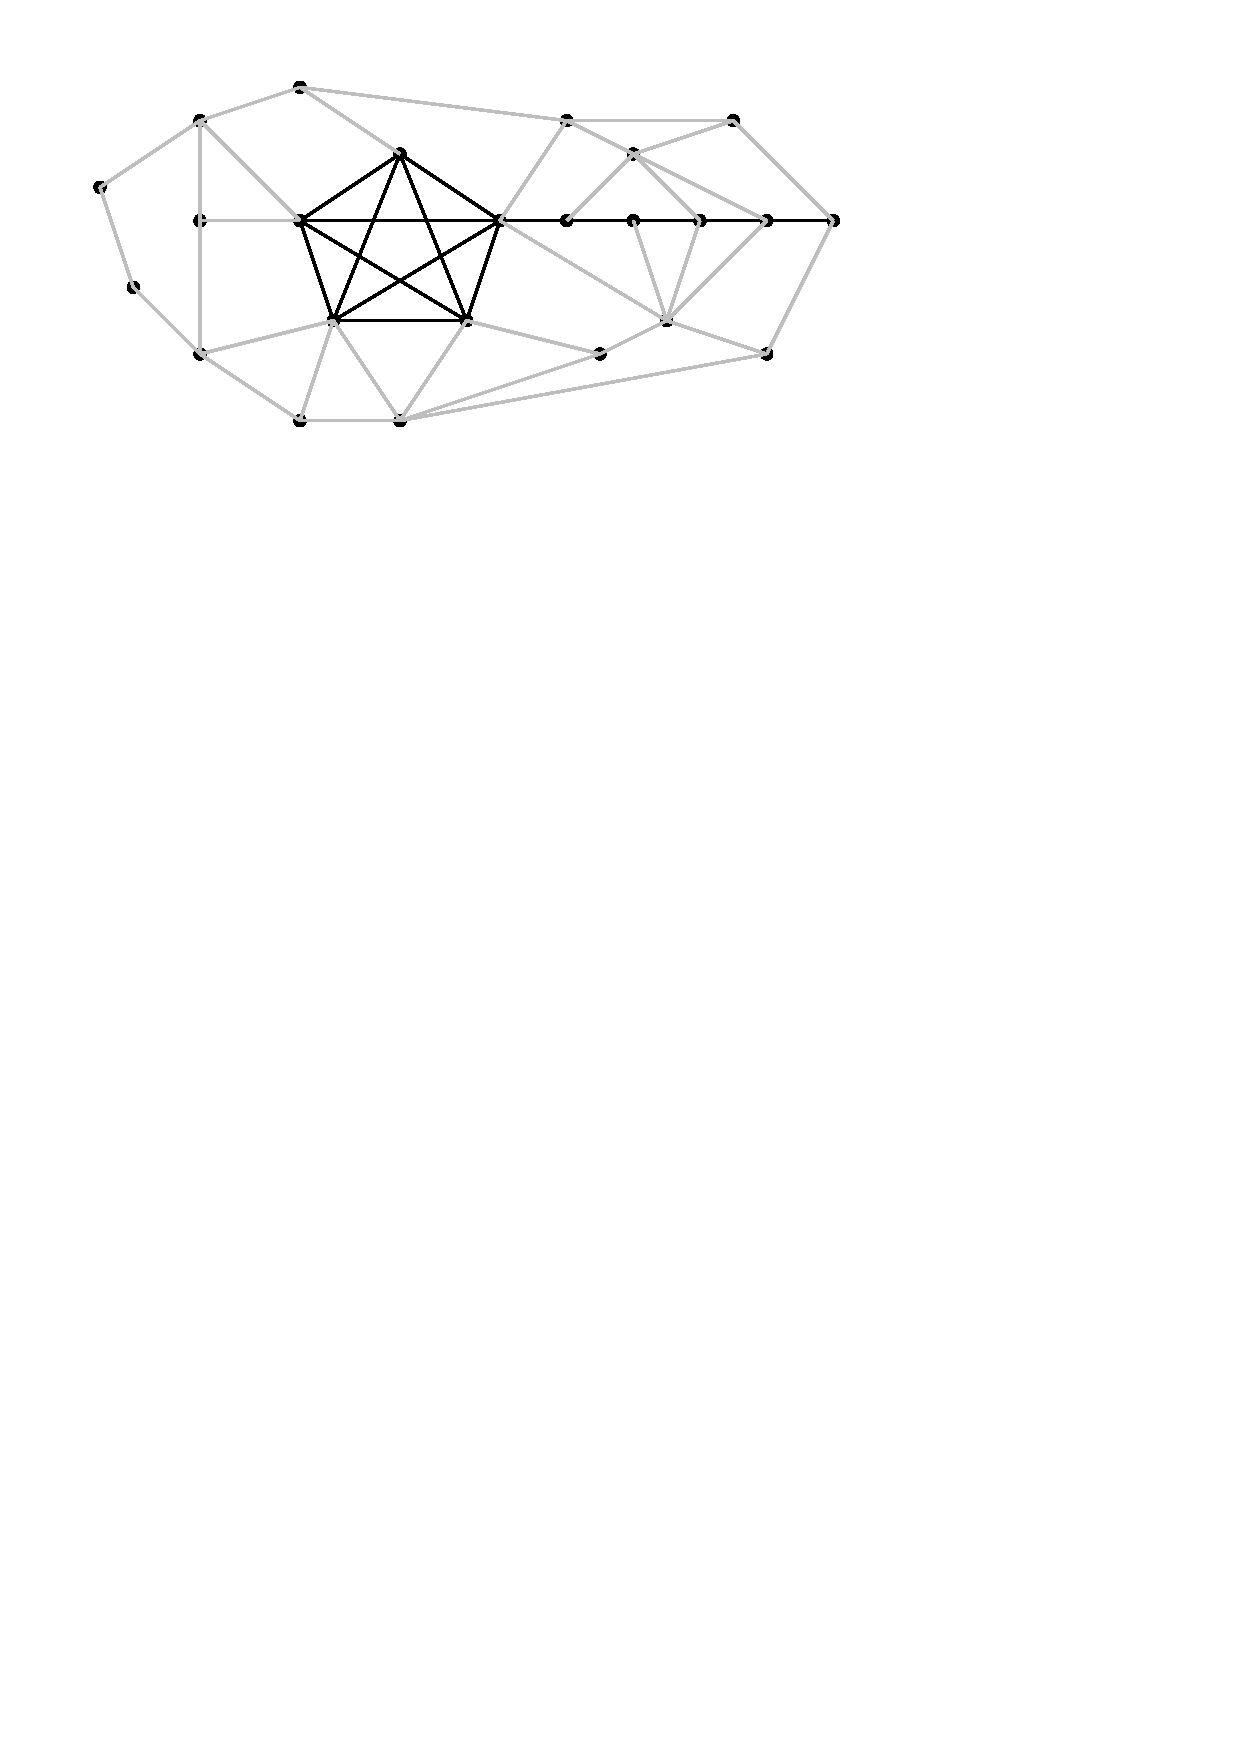
\includegraphics[scale=0.5]{kite}
\end{center}

The \emph{kite problem} is defined as follows:
\[ \KITE = \{ (G,K) : \mbox{ graph $G$ contains a $K$-kite} \} . 
\]

\noindent
Prove that the language $\KITE$ is in {\bf NP}.
\end{question}

\begin{solution}
      
      To prove that KITE is in NP, we need to show that there is a polynomial-time algorithm
      that can verify this.

      To verify whether or not (G,K) is in KITE we can do these steps:

      1. Check if G contains a clique of size K by checking all possible subsets
      of K vertices in G and seeing whether they form a complete subgraph or not.

      2. If G does not contain a clique of size K, (G,K) cannot be KITE.

      3. Otherwise, choose a vertex in the clique and check if
      there is a path of K vertices in G that is connected to that vertex,
      by exploring all paths of length K that start at the vertex.

      4. If there exists a path of K vertices in G that is connected to that
      vertex, then (G,K) is in KITE, otherwise it is not.

      The runtime of this is in polynomial time, therefore, KITE is in NP.

\end{solution}

\begin{question}
The \emph{clique problem} is defined as follows:
\[ \CLIQUE= \{ (G,K) : \mbox{ graph $G$ contains a clique of size $K$} 
            \} . 
\]
Prove that $\CLIQUE \leq_P \KITE$, i.e., in polynomial time, $\CLIQUE$ 
can be reduced to $\KITE$.
\end{question}

\begin{solution}
      
      To prove that $\CLIQUE \leq_P \KITE$, we need to show that there is a
      polynomial-time reduction from Clique to Kite. We need to show that given
      (G,K) of Clique, we can construct (G',K') of Kite such that (G,K) is in Clique
      if and only if (G',K') is in Kite.

      Construction of G':
      
      For each vertex v in G, add a new vertex to G' and connect it to the
      vertex in G' to form a path of length 1.
      Then create a new vertex and connect it all to the vertices to form a clique.

      The resulting new graph should have 2K vertices and constructed in polynomial time.
      G' contains a K-kite if and only if G contains a clique of size K.

      Suppose that (G',2K) is an instance of Kite, then the clique in the K-kite must include
      the new vertex and at least K - 1 vertices from before. Let S be the set of corresponding
      vertices in G, then S forms a clique of size K in G, thus G contains a clique of size K.

      Therefore, the reduction algorithm constructs (G',2K) of Kite from (G,K) of Clique
      in polynomial time, and (G,K) is in Clique if and only if (G',2K) is in Kite, and
      $\CLIQUE \leq_P \KITE$.
\end{solution}

\begin{question}
The \emph{subset sum problem} is defined as follows:

\vspace{0.5em}

\begin{tabular}{rl}
   $\SubSum = \{ (S,t) :$ & $S$ is a set of integers, $t$ is 
                            an integer, \\ 
                     & $\exists S' \subseteq S$ such that 
                       $\sum_{x \in S'} x = t$ $\}$.
\end{tabular}

\vspace{0.5em}

\noindent 
The \emph{partition problem} is defined as follows:

\vspace{0.5em}

\begin{tabular}{rl}
   $\Partition = \{ S :$ & $S$ is a set of integers, \\ 
                     & $\exists S' \subseteq S$ such that 
                       $\sum_{x \in S'} x = 
                        \sum_{y \in S \setminus S'} y$ $\}$.
\end{tabular}

\begin{itemize} 
\item Prove that $\SubSum \leq_P \Partition$, i.e., in polynomial time, 
$\SubSum$ can be reduced to $\Partition$.
\item Prove that $\Partition \leq_P \SubSum$, i.e., in polynomial time, 
$\Partition$ can be reduced to $\SubSum$.
\end{itemize} 
\end{question}

\begin{solution}
      
      To prove that $\SubSum \leq_P \Partition$, i.e., in polynomial time, 
      $\SubSum$ can be reduced to $\Partition$, we need to construct S' of Partition.

      Given (S,t), we construct S':

      First we compute the sum of all the elements in S and we can call that sum(S).
      Next we double every element in S and let that be S'. Now we compute the sum of all elements
      in S' and label that sum(S'). Now if t $>$ sum(S') then add (t - sum(S')) to S' as a new element,
      otherwise we add (sum(S') - t) to S' as new element.

      Now we suppose that (S, t) is an instance of SubsetSum. 
      Then there exists a subset S'' $\subseteq$ S such that the sum of the elements in S'' is equal to t. 
      Let S''' = {2x : x $\in$ S''}. 
      Then the sum of the elements in S''' is equal to 2t. 
      Since S' contains all the elements of S''' and possibly one more element, 
      the sum of the elements in S' is equal to 2t + a, where a is either 0 or $|t - sum(S')|$. 
      Therefore, S' is an instance of Partition.

      We now suppose that S' is an instance of Partition. 
      Then there exists a subset S'' $\subseteq$ S' such that the sum of the elements in S'' is equal to sum(S')/2 (if sum(S') is odd, 
      then we consider the closest integer to sum(S')/2). Let S''' = {x/2 : x $\in$ S''}. Then the sum of the elements in S''' is equal to sum(S)/2. 
      Since S''' is a subset of S, the sum of the elements in S''' is also equal to t, which means that (S, t) is an instance of SubsetSum.

      Therefore, reduction is correct and $\SubSum \leq_P \Partition$.

      \vspace{0.5em} 

      We will now prove that $\Partition \leq_P \SubSum$, i.e., in polynomial time, 
      $\Partition$ can be reduced to $\SubSum$

      Given S, we will need to construct (S',t):

      We need to compute the sum of all elements in S and label it sum(S) again.
      Then we compute sum(S)/2 and set that equal to t. Lastly, we let S' be S.

      First, suppose that S is an instance of Partition. 
      Then there exists a subset S'' $\subseteq$ S such that the sum of the elements in S'' is equal to sum(S)/2. 
      Since t is equal to sum(S)/2, the sum of the elements in S'' is also equal to t. 
      Therefore, (S', t) is an instance of SubsetSum.

      Now we suppose that (S', t) is an instance of SubsetSum. 
      Then there exists a subset S'' $\subseteq$ S' such that the sum of the elements in S'' is equal to t. 
      Since S' = S, the sum of the elements in S'' is also equal to sum(S)/2. 
      Therefore, S is an instance of Partition.

      Therefore, reduction is correct and $\Partition \leq_P \SubSum$.
\end{solution}

\begin{question}
The \emph{clique and independent set problem} is defined as follows:

\vspace{0.5em} 

\begin{tabular}{rl}
   $\CLIS= \{ (G,K) :$ & graph $G$ contains a clique of size $K$ and \\  
                       & $G$ contains an independent set of size $K$  
                         $\}$.
\end{tabular}

\vspace{0.5em} 

\noindent 
Prove that $\CLIQUE \leq_P \CLIS$, i.e., in polynomial time, 
$\CLIQUE$ can be reduced to $\CLIS$.
\end{question}

\begin{solution}
      
      Given an instance of Clique (G,K), we need to construct an instance
      of the CliqueIndepSet (G',K') such that G contains a clique of size 
      K if and only if G' contains a clique of size K' and an independent
      set of size K'.

      Construction:
      Let G' be the complement of G, i.e., the graph with the same vertex set as G, 
      but with an edge between any two vertices that are not connected by an edge in G. 
      Clearly, a clique of size k in G corresponds to an independent set of size k in G'. 
      Similarly, an independent set of size k in G corresponds to a clique of size k in G'. 
      Therefore, if we set K' = $|V(G)| - K$, then G contains a clique of size K 
      if and only if G' contains a clique of size K' and an independent set of size K'.
      The construction is done in polynomial time. Therefore, the reduction
      from Clique to CliqueIndepSet is in polynomial-time, $\CLIQUE \leq_P \CLIS$.
\end{solution}

\newpage

\begin{question}
Let $\varphi$ be a Boolean formula in the variables
$x_1,x_2,\ldots,x_n$. We say that $\varphi$ is in 
\emph{conjunctive normal form} (CNF) if it is of the form
\[ \varphi = C_1 \wedge C_2 \wedge \ldots \wedge C_m ,
\]
where each $C_i$, $1 \leq i \leq m$, is of the following form:
\[ C_i = l_1^i \vee l_2^i \vee \ldots \vee l_{k_i}^i .
\]
Each $l_j^i$ is a \emph{literal}, which is either a variable or the
negation of a variable.

The \emph{satisfiability problem} is defined as follows:
\[ \SAT = \{ \varphi : \varphi \mbox{ is in CNF-form
                                       and is satisfiable} \} .  
\]

\noindent
Prove that $\CLIQUE \leq_P \SAT$, i.e., in polynomial time, $\CLIQUE$ 
can be reduced to $\SAT$.
\end{question}

\begin{solution}
      
      Given an instance of Clique (G,K), 
      we need to construct an instance of the satisfiability problem, 
      which is a Boolean formula in CNF-form $\varphi$ such that G contains a 
      clique of size K if and only if $\varphi$ is satisfiable.

      Let $V = {v_1, v_2, ..., v_n}$ be the set of vertices of G. 
      For each vertex $v_i$, introduce a Boolean variable $x_i$. 
      We will construct a Boolean formula $\varphi$ in CNF-form that is satisfiable if and only if G has a clique of size K.

      First, add the clauses ($x_i$ $\lor$ $x_j$) for every pair of vertices i, j that are connected by an edge in G. This ensures that if two vertices are connected, at least one of them must be in any clique.

      Next, add the clauses $\neg x_i$ $\lor$ $\neg x_j$ for every pair of vertices i, j that are not connected by an edge in G. This ensures that if two vertices are not connected, both of them cannot be in any clique.

      Finally, add the clauses ($x_{i1}$ $\lor$ $x_{i2}$ $\lor$ ... $\lor$ $x_{ik}$) for every k-clique in G. This ensures that at least k vertices in the clique must be true, which is only possible if the corresponding Boolean variables are set to true.

      Construction is done is polynomial-time, therefore, $\CLIQUE \leq_P \SAT$.
\end{solution}

\end{document} 